% Diagrama de estados de la Práctica 5 (fsm_p5.cpp). Compilar: pdflatex diagrama-estados-p5.tex
\documentclass[tikz,border=6pt]{standalone}
\usepackage[utf8]{inputenc}
\usepackage[T1]{fontenc}
\usepackage{lmodern}
\usetikzlibrary{arrows.meta,positioning}
\definecolor{optoemit}{HTML}{C9601F}
\definecolor{optoalert}{HTML}{B23A34}
\definecolor{optodetect}{HTML}{6B4C9A}
\definecolor{optoink}{HTML}{1C1F24}
\definecolor{optoconfirm}{HTML}{3E7C59}
\begin{document}
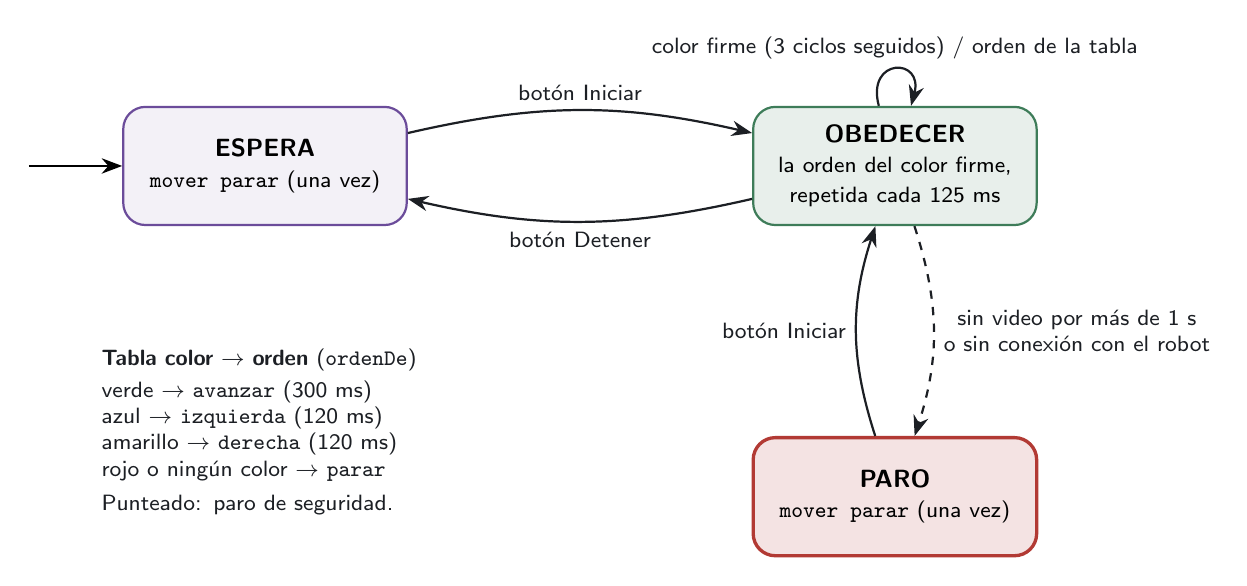
\begin{tikzpicture}[font=\sffamily\small, >={Stealth[length=2.6mm]},
  e/.style={draw=optoink, thick, rounded corners=8pt, minimum width=3.6cm, minimum height=1.5cm, align=center, fill=white},
  t/.style={font=\sffamily\footnotesize, align=center, text=optoink},
  tr/.style={->, thick, optoink}]
\node[e, draw=optodetect, fill=optodetect!8] (espera) at (0,0) {\textbf{ESPERA}\\\footnotesize\texttt{mover parar} (una vez)};
\node[e, draw=optoconfirm, fill=optoconfirm!12] (obedecer) at (8,0) {\textbf{OBEDECER}\\\footnotesize la orden del color firme,\\\footnotesize repetida cada 125 ms};
\node[e, draw=optoalert, very thick, fill=optoalert!14] (paro) at (8,-4.2) {\textbf{PARO}\\\footnotesize\texttt{mover parar} (una vez)};
\draw[->, thick] (-3.0,0) -- (espera);
\draw[tr] (espera) to[bend left=13] node[t, above]{botón Iniciar} (obedecer);
\draw[tr] (obedecer) to[bend left=13] node[t, below]{botón Detener} (espera);
\draw[tr, dashed] (obedecer) to[bend left=18] node[t, right]{sin video por más de 1 s\\o sin conexión con el robot} (paro);
\draw[tr] (paro) to[bend left=18] node[t, left]{botón Iniciar} (obedecer);
\draw[tr] (obedecer) edge[loop above, looseness=4] node[t, above]{color firme (3 ciclos seguidos) / orden de la tabla} (obedecer);
\node[t, anchor=north west, text width=6.6cm, align=left] at (-2.2,-2.2) {\textbf{Tabla color $\rightarrow$ orden} (\texttt{ordenDe})\\[2pt]
verde $\rightarrow$ \texttt{avanzar} (300 ms)\\azul $\rightarrow$ \texttt{izquierda} (120 ms)\\amarillo $\rightarrow$ \texttt{derecha} (120 ms)\\rojo o ningún color $\rightarrow$ \texttt{parar}\\[3pt]
Punteado: paro de seguridad.};
\end{tikzpicture}
\end{document}
